%!TEX root=/home/ska124/Dropbox/Thesis/thes-full.tex

%%%%%%%%%%%%%%%%%%%%%%%%%%%%%%%%%%%%%%%%%%%%%%%%%
%
%     Chapter 4   
%
%%%%%%%%%%%%%%%%%%%%%%%%%%%%%%%%%%%%%%%%%%%%%%%%

\chapter{Implementation}
\label{chap:hardware_complexity_and_simulation}

This chapter describes the additional hardware complexity added to an \AC\ with respect to a conventional cache in order to support variable granularity \AB{}s. The chapter also describes the simulation infrastructure used to evaluate the performance of the \AC{}.

\section{Hardware complexity}  
\label{sec:hardware_complexity}

The complexity of the \AC\ is analysed along the following directions:
\begin{itemize}
  \item Additional complexity of the cache controller
  \item Area, latency and energy overhead
  \item Challenges of megabyte sized \AC{}s
\end{itemize}


\subsection{Cache Controller} 

Each level of the cache memory hierarchy incorporates a finite state machine (FSM) called the \textit{cache controller} to track the state of the blocks currently being cached. The cache controller is the interface between the CPU, cache and DRAM as shown in Fig~\ref{fig:cache_controller_basics}(a). The figure depicts a look through hierarchy where the processor is isolated from the system, thus allowing the processor to run with data from the cache while another bus master is acessing main memory. Fig~\ref{fig:cache_controller_basics}(b) shows an overview of the implementation logic for the cache controller. Using the current state of the block and the incoming request ( which could be from the CPU, DRAM or a remote cache) a new state is set for the cache block. The state transition diagram of an L1 \AC\ is shown in Fig~\ref{fig:L1protocol}. The FSM for the \AC\ is a superset of an equivalent FSM for a conventional cache (without cache coherence; more details in \S~\ref{sec:coherence}).

\begin{figure}[h]
  \subfloat[Interface]{
    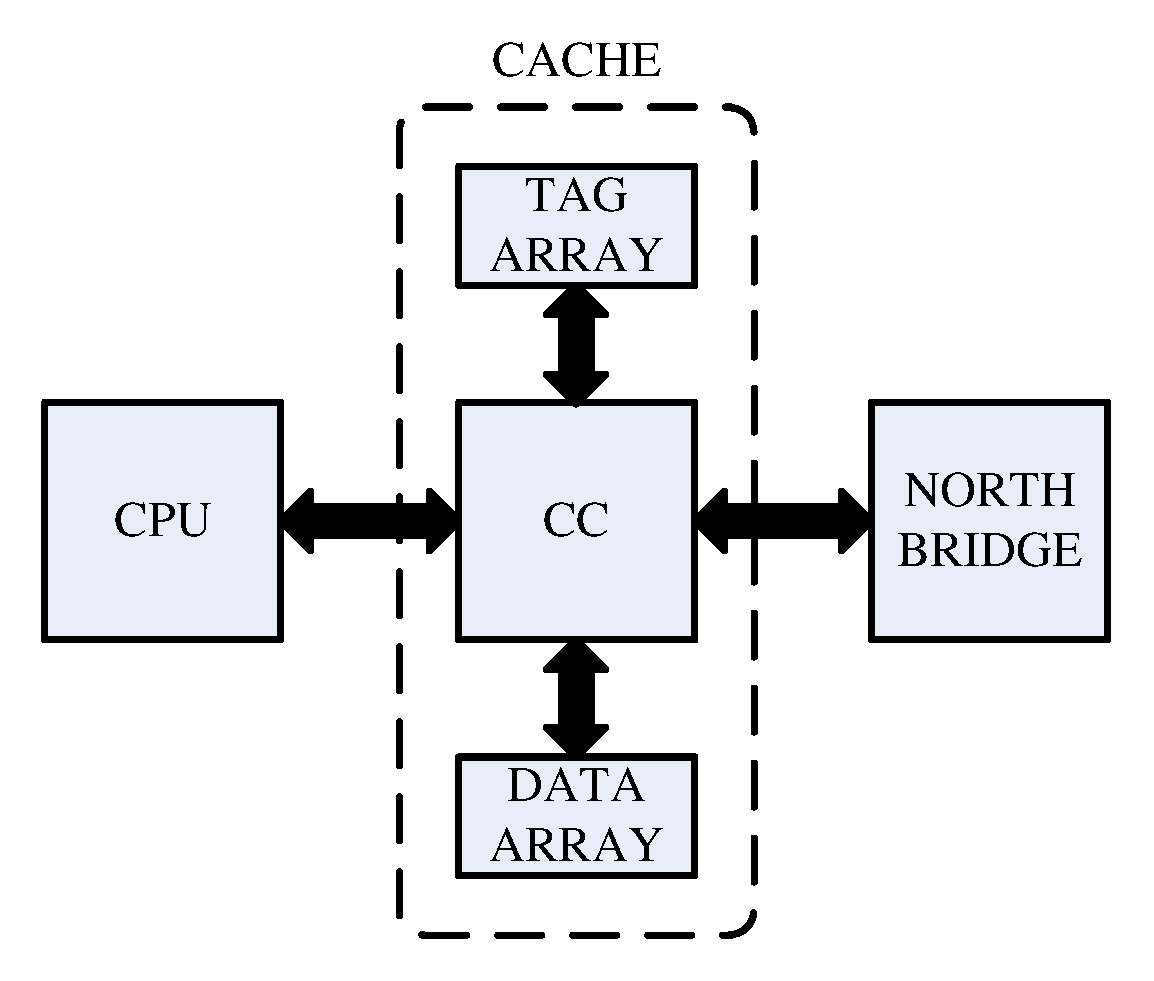
\includegraphics[width=0.5\textwidth]{files/Figures/07-LookThroughArchitecture.pdf}
  }
  \subfloat[FSM Logic]{
     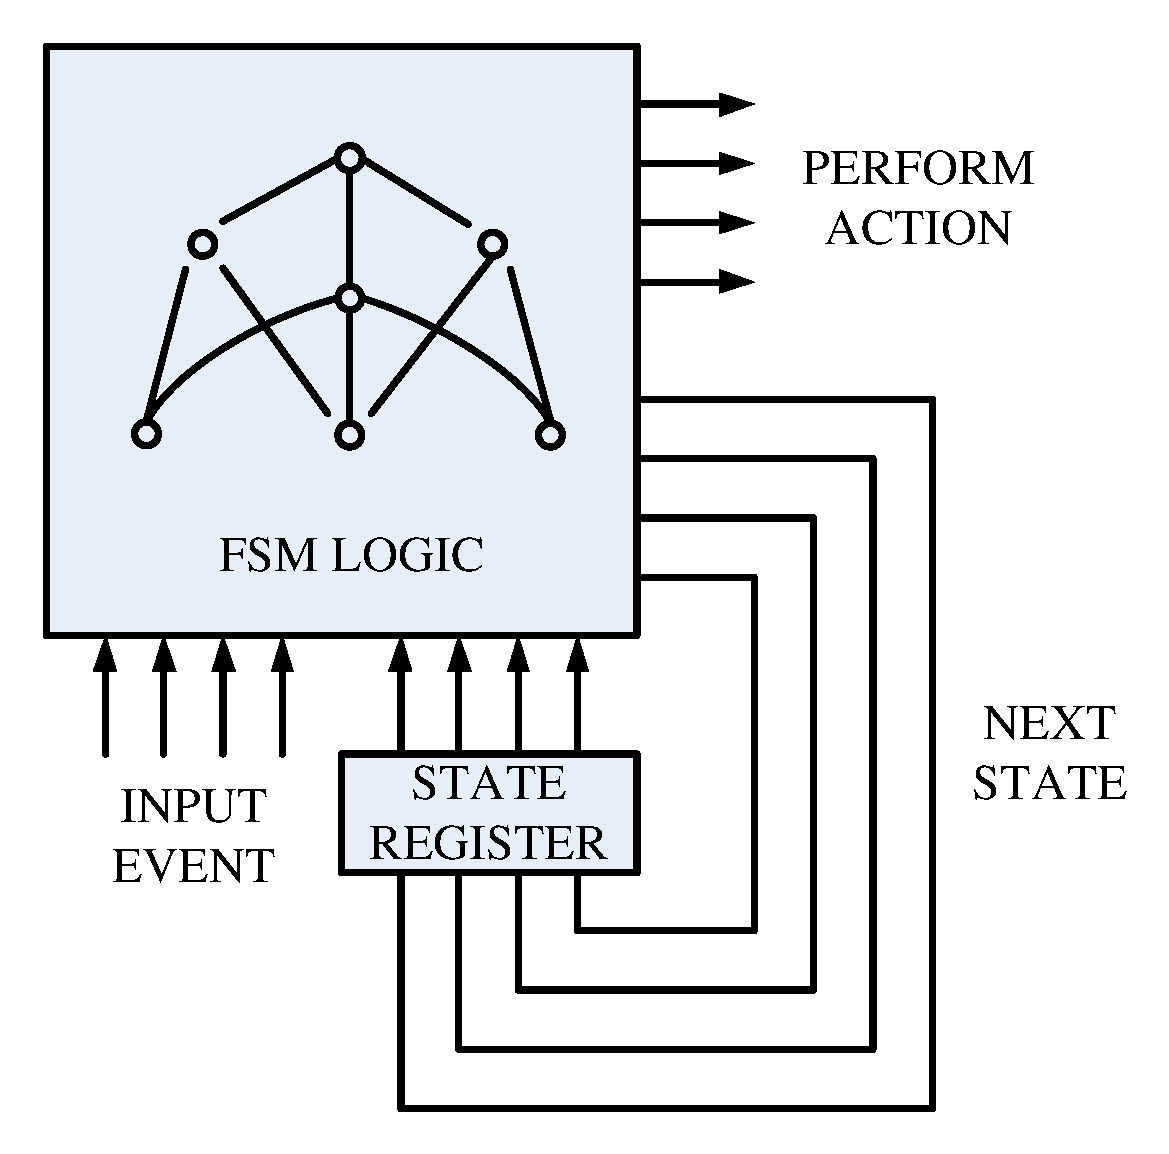
\includegraphics[width=0.5\textwidth]{files/Figures/07-FSMLogic.pdf}
  }
  \caption[Cache Controller]{Fig (a) on the left shows a high level block diagram of the cache controller's (CC) position in the memory hierarchy. The \textit{Northbridge} is used to manage data communcations between the CPU and motherboard and is also where the memory controller resides. In newer architectures such as the Intel Sandy Bridge, the \textit{Northbridge} has been integrated on chip. Fig (b) on the right depicts a cache controller where the input data path from the cache (event) is used along with the current state to perform the corresponding action and change the state of the block as required.}
  \label{fig:cache_controller_basics}
\end{figure}


The cache controller manages operations at the aligned RMAX granularity. The controller permits only one in-flight cache operation per RMAX region, i.e. transition buffer entries in the cache controller are indexed using the region bits. In-flight cache operations ensure no address overlap with stable \AB{}s in order to eliminate complex race conditions. Fig~\ref{fig:L1protocol} shows the L1 cache controller state machine for the \AC{}. 

\begin{figure}[!h]
  \centering
  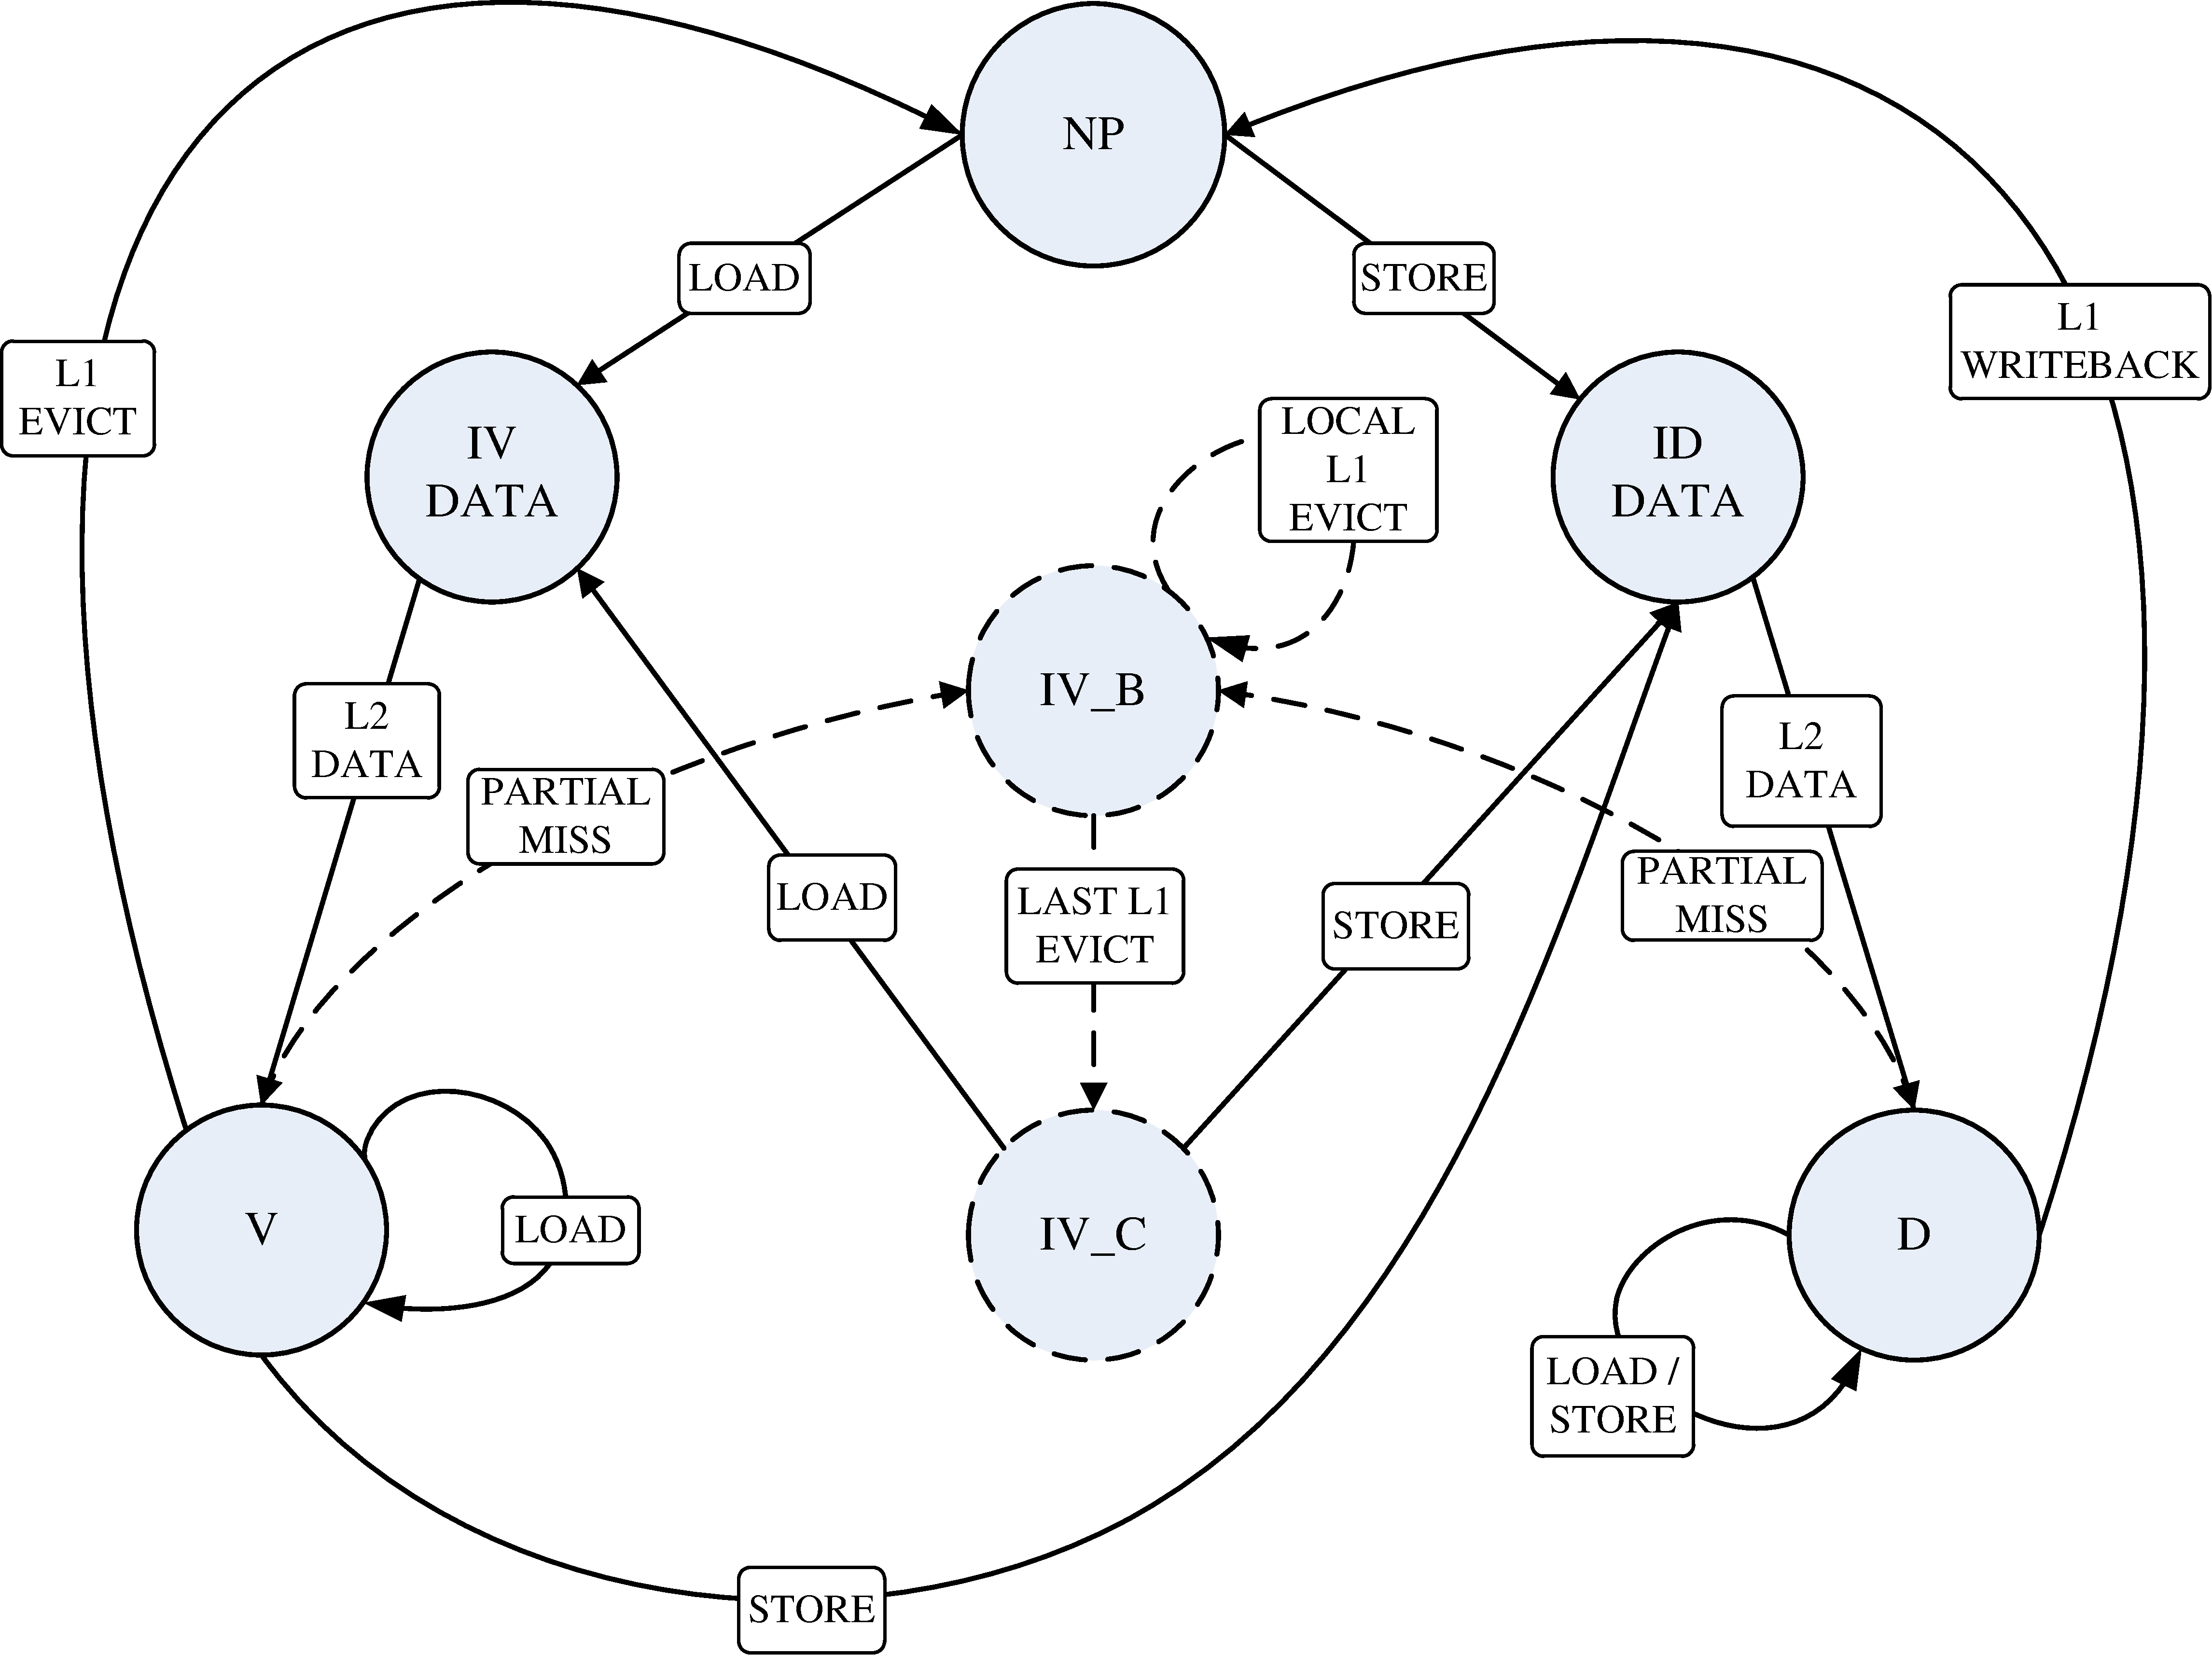
\includegraphics[width=\textwidth]{files/Figures/07-L1CC.pdf}
  \\ 
  \vspace{10pt}
  {
  \begin{tabular}{|@{~}c@{~}|@{~}p{0.75\textwidth}|} 
        
        \multicolumn{2}{c}{ \textbf{L1 cache controller states}}\\
        \hline
        State & Description \\
        \hline
        NP & \AB\ not present in the cache. \\
        \hline
        V & All words corresponding to \AB\ present and valid (read-only) \\
        \hline
        D & Valid and atleast one word in \AB\ is dirty (read-write) \\
        \hline
        {\bf IV\_B} & Partial miss being processed (blocking state) \\
        \hline
        {\bf IV\_Data} & Load miss; waiting for data from L2\\
        \hline
        ID\_Data & Store miss; waiting for data. Set dirty bit. \\
        \hline
        {\bf IV\_C} & Partial miss cleanup from cache completed (treat as full miss) \\ 
        \hline
        \multicolumn{2}{c}{}\\
        \multicolumn{2}{c}{ \textbf{ \AC\ specific events}}\\
        \hline
        \multicolumn{2}{|p{5in}|}{Partial miss: Process partial miss.} \\
        \multicolumn{2}{|p{5in}|}{Local\_L1\_Evict: Remove overlapping \AB\ to MSHR.} \\
        \multicolumn{2}{|p{5in}|}{Last\_L1\_Evict: Last \AB\ moved to MSHR. Convert to full miss and process load or store.} \\
        \hline
    \end{tabular}
    }
  \caption[L1 Cache Controller]{\textbf{L1 Cache Controller for \AC\ } : The \AC\ specific states and events are marked by dashed lines. The \AC\ specific events are described in the table.}
  \label{fig:L1protocol}
\end{figure}

\clearpage

A simple default single core protocol is assumed which contains blocks in either \code{Valid (V)}, \code{Not Present (NP)} and \code{Dirty (D)} as shown in Fig~\ref{fig:L1protocol}. There are also two transient states \code{IV Data}(block transitions from \code{Invalid/NP} to \code{Valid}, waiting for \code{Data} response from memory; cache miss caused by a load) and \code{ID Data}(block transitions from \code{Invalid/NP} to \code{Dirty}, waiting for \code{Data} response from memory; cache miss caused by a store). To handle partial misses, unique to the \AC{}, two new states are added to the default protocol, \code{IV\_B} and \code{IV\_C}. \code{IV\_B} is a blocking state that blocks other cache operations to RMAX region until all relevant \AB{}s to a partial miss are evicted. \code{IV\_C} indicates partial miss completion. This enables the controller to treat the access as a miss and issue the refill request. The \code{Partial Miss} event triggers the clean-up operations (Stage 1 and Stage 2 in Figure~\ref{fig:partial-miss}). \code{Local\_L1\_Evict} is an event that keeps being triggered for each \AB\ involved in the partial miss. \code{Last\_L1\_Evict} is triggered when the last \AB\ involved in the partial miss is evicted to the MSHR (see Stage 2 of Fig~\ref{fig:partial-miss}).

A key difference between the L1 and lower-level protocols is that the Load/Store event in the lower-level protocol may need to access data from multiple \AB{}s. In such cases, similar to the \code{Partial Miss} event, each block is read out independently before supplying the data (more details in \S~\ref{sec:multicache}).

\subsection{Area, latency, and energy Overhead}
\label{sec:area_latency_energy_overhead}

The extra metadata required by \AC\ are the \code{T?}(1 tag bit per word) and \code{V?}(1 valid bit per word) bitmaps as shown in Fig~\ref{fig:amoeba_cache_arch}. Table~\ref{table:overheads} shows the quantitative overhead compared to the data storage.Both the \code{T?} and \code{V?} bitmap arrays are directly proportional to the size of the cache and require a constant storage overhead (3\% in total). The \code{T?} bitmap is read in parallel with the data array and does not affect the critical path; \code{T?} adds 2\%---3.5\% (depending on cache siz) to the overall cache access energy. \code{V?}is referred only on misses when inserting a new block.

%!TEX root=/home/ska124/Dropbox/Thesis/thes-full.tex

\begin{table}[h]
{
  \centering
  
  
  {
  
    \begin{tabular}{|@{~}c@{~}|@{~}c@{~}|@{~}c@{~}|@{~}c@{~}|}
    \hline
    \multicolumn{4}{|c|}{Cache configuration}\\
    \hline
                 & 64K (256by/set) & 1MB (512by/set) & 4MB (1024by/set) \\
    \hline
    \multicolumn{4}{|l|}{Data RAM parameters} \\   
    \hline
    Delay        & 0.36ns & 2ns & 2.5 ns \\
    Energy       & 100pJ & 230pJ  & 280pJ \\
    \hline 
    \multicolumn{4}{|c|}{\AC\ components (CACTI model)} \\   
    \hline
    T?/V? map & 1KB &  16KB & 64KB \\
    Latency      & 0.019ns (5\%) & 0.12ns (6\%) & 0.2ns (6\%) \\   
    Energy       & 2pJ (2\%) & 8pJ (3.4\%) & 10pJ (3.5\%)  \\ 
    LRU  & $\frac{1}{8}$KB & 2KB & 8KB \\
    \hline
    \multicolumn{4}{|c|}{Lookup Overhead (VHDL model)} \\
    \hline
    Area    & 0.7\% & \multicolumn{2}{c|}{0.1\%} \\  
    \hline
    Latency & 0.02ns & 0.035ns & 0.04ns \\
    \hline
  \end{tabular}
  }
  \caption[Hardware Overheads]{\textbf{\AC\ hardware overheads} :  Percentage indicates overhead compared to data array of a cache. 64K cache operates in \textit{Fast mode}; 1MB and 4MB operate in \textit{Normal mode}. International Technology Roadmap for Semiconductors (ITRS) specified 32nm High Performance (HP) transistors are assumed for 64K cache and 32nm ITRS Low Output Power (LOP) transistors for 1MB and 4MB.}
  \label{table:overheads}
}
\end{table}

The \AC\ lookup logic was synthesized\footnote{Actual synthesis was at 180nm node size and the results were scaled to 32 nm (latency and energy scaled proportional to Vdd (taken from~\cite{Danowitz:2012:CDR:2133806.2133822}) and $Vdd^2$ respectively). For synthesis, we used the Synopsys design compiler (Vision Z-2007.03-SP5).} using Synopsys to quantify the area, latency and energy penalty. \AC\ is compatible with  \textit{Fast} and \textit{Normal} cache access modes~\cite{Muralimanohar:2007:ONO:1331699.1331704}, both of which read the entire set from the data array in parallel with the way selection to  achieve lower latency. \textit{Fast} mode transfers the entire set to the edge of the H-tree, while \textit{Normal} mode, only transmits the selected way over the H-tree. 

Fig~\ref{fig:ac_lookup} shows \AC\'s lookup hardware overhead on the critical path. The \AC\ lookup logic is compared against a conventional cache's lookup logic (mainly the comparators). The area overhead of the \AC\ includes registering an entire line that has been read out, the tag operation logic, and the word selector. The components on the critical path once the data is read out are the 2-way multiplexers, the $\in$ comparators, and priority encoder that selects the word; the T?  bitmap is accessed in parallel and off the critical path. \AC\ is made feasible under today's wire-limited technology where the cache latency and energy is dominated by the bit/word lines, decoder, and H-tree~\cite{Muralimanohar:2007:ONO:1331699.1331704}. \AC{}'s comparators, which operate on the entire cache set, are 6$\times$ the area of a fixed cache's comparators. In a conventional cache, the data array occupies 99\% of the overall cache area. The critical path is dominated by the wide word selector since the comparators all operate in parallel. The lookup logic adds $\simeq$ 60\% to the conventional cache's comparator time. The overall critical path is dominated by the data array access and \AC{}'s lookup circuit adds 0.02ns to the access latency and $\simeq$ 1pJ to the energy of a 64K cache, and 0.035ns to the latency and $\simeq$2pJ to the energy of a 1MB cache. 

\AC{}'s overhead needs careful consideration when implemented at the L1 cache level. There are two options for handling the latency overhead a) if the L1 cache is the critical stage in the pipeline, the CPU clock can be throttled by the latency overhead to ensure that the additional logic fits within the pipeline stage. This ensures that the number of pipeline stages for a memory access does not change with respect to a conventional cache, although all instructions bear the overhead of the reduced CPU clock; b) an extra pipeline stage can be added to the L1 hit path, adding a 1 cycle overhead to all memory accesses but ensuring no change in CPU frequency. The performance impact of both approaches is quantified in \S~\ref{sec:evaluation}.


\subsection{Tag-only operations}  

Conventional caches support tag-only operations to reduce data port contention. While the \AC\ merges tags and data, like many commercial processors it decouples the replacement metadata and valid bits from the tags, accessing the tags only on cache lookup. Lookups can be either CPU side or network side (coherence invalidations, writebacks or forwarding). CPU-side lookups and writebacks ($\simeq$ 95\% of cache operations) both need data and hence \AC\ in the common case does not introduce extra overhead. \AC\ does read out the entire data array unlike serial-mode caches as discussed previously. Invalidation checks and snoops can be more energy expensive with \AC{} compared to a conventional cache. Fortunately, coherence snoops are not common in many applications (e.g., 1/100 cache operations in SpecJBB) as a coherence directory and an inclusive LLC filter them out.


\subsection{Tradeoff with large caches} 
\label{sec:tradeoff_with_large_caches} % formerly extensions

\begin{figure}[h] 
\centering
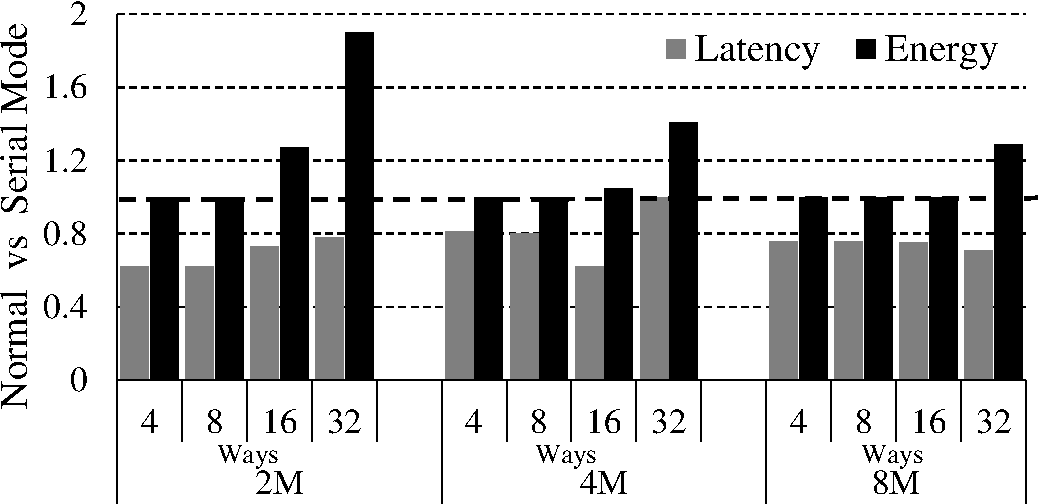
\includegraphics[width=0.7\textwidth]{files/Plots/07-Serial_vs_Normal.pdf}

Baseline: Serial. $\leq1$ Normal is better.  32nm, ITRS  LOP. 
\caption[Serial vs. Normal - Latency and Energy]{\textbf{Serial vs Normal mode cache} : This graph shows the ratio of Serial mode access versus Normal mode access. Thus values less than 1 indicate the serial mode access is more efficient. The cache configurations are grouped in terms of size and subgroups for the number of ways per cache set. }
\label{fig:serial_normal_graph} 
\end{figure}

Large caches with many words per set ($\equiv$ highly associative conventional cache) need careful consideration. Typically, highly associative caches tend to serialize tag and data access with only the relevant cache block read out on a hit and no data access on a miss. The tradeoff between reading the entire set (normal mode), which is compatible with \AC{}, and only the relevant block (serial mode), is analysed herein. The cache size is varied from 2M---8M and associativity from 4(256B/set) --- 32 (2048B/set). Under current technology constraints (Figure~\ref{fig:serial_normal_graph}), only at very high associativity does serial mode demonstrate a notable energy benefit. Large caches are dominated by H-tree energy consumption and reading out the entire set at each sub-bank imposes an energy penalty when bitlines and wordlines dominate (more than 2KB of words per set).

\begin{table}[h]
\begin{center}
\begin{tabular}{|c|c|c|c|c|c|c|}
\hline
  &  \multicolumn{2}{c|} {64K (256 bytes/set)} 
  &  \multicolumn{2}{c|} {1MB (512 bytes/set)} 
  & \multicolumn{2}{c|} {2MB (1024 bytes/set)} \\
\hline
N Tags/set & 2 & 4 & 4 & 8 & 8 & 16 \\
Overhead &  1KB & 2KB  & 2KB & 16KB  & 16KB & 32KB  \\  
\hline
\multicolumn{7}{|l|} {Benchmarks} \\
\hline
Low      & 30\% & 45\% & 42\% & 64\% & 55\% & 74\%\\
Moderate & 24\% & 62\% & 46\% & 70\% & 63\% & 85\%\\
High     & 35\% & 79\% & 67\% & 95\% & 75\% & 96\%\\
\hline
\end{tabular}
\caption[Fast Tag accesses percent]{Percentage of direct accesses with fast tags}
\label{fig:tagcount}

\end{center}
\end{table}


The \AC\ can be tuned to minimize the hardware overhead for large caches. With many words/set the cache utilization improves due to longer block lifetimes making it feasible to support \AB{}s with a larger minimum granularity ($>$ 1 word). If we increase minimum granularity to two or four words, only every third or fifth word could be a tag, thus the number of comparators and multiplexers required for lookup reduce to $\frac{N_{words/set}}{3}$ or $\frac{N_{words/set}}{5}$. When the minimum granularity is equal to max granularity (RMAX), we obtain a fixed granularity cache with $N_{words/set}/RMAX$ ways. Cache organizations that collocate all the tags together at the head of the data array enable tag-only operations and serial \AB\ accesses that need to activate only a portion of the data array. However, the set may need to be compacted at each insertion. Recently, Loh and Hill~\cite{Loh:2012:SVL:2311639.2311823} explored such an organization for supporting tags in multi-gigabyte caches.

The use of \textit{Fast Tags} help reduce the tag lookups in the data array. Fast tags use a separate traditional tag array-like structure to cache the tags of the recently-used blocks and provide a pointer directly to the \AB{} similar to \textit{Indirect Index Caches}(see \S~\ref{sec:indirect_index_caches}). The number of \textit{Fast Tags} needed per set is proportional to the number of blocks in each set, which varies with the spatial locality in the application and the number of bytes per set (more details in Section~\ref{sec:efficiency}). Three different cache configurations were studied (64K 256B/set, 1M 512B/set, and 2M 1024B/set) while varying the number of fast tags per set (see Table~\ref{fig:tagcount}). With 8 tags/set (16KB overhead), the fast tags can filter 64---95\% of the accesses in a 1MB cache and 55---75\% of the accesses in a 2MB cache.

\subsection{Hierarchical cache memory systems}
\label{sec:multicache}

The \AC\ can be implemented in a hierarchical cache memory system of \textit{Inclusive} nature (see \S~\ref{sec:cache_memory_systems}). For the \AC\ however, inclusion means that the L2 cache contains a superset of the data words in the L1 cache; however, the two levels may include different granularity blocks. For example, the Sun Niagara T2 uses 16 byte L1 blocks and 64 byte L2 blocks. \AC\ permits non-aligned blocks of variable granularity at the L1 and the L2, and needs to deal with two issues: a) L2 events that may invalidate multiple L1 blocks and b) L1 refills that may need data from multiple blocks at the L2. For both cases, the \AC\ needs to identify all the relevant \AB{}s that overlap with either the recall or the refill request. This situation is similar to a Nigara's L2 eviction which may need to recall 4 L1 blocks. \AC{}'s logic ensures that all \AB{}s from a region map to a single set at any level (using the same RMAX for both L1 and L2). This ensures that L2 recalls or L1 refills index into only a single set. To process multiple blocks for a single cache operation, the \AC\ uses the step-by-step process outlined in \S~\ref{sec:partialmiss} (Stage 1 and Stage 2 in Fig~\ref{fig:partial-miss}). Finally, the L1-L2 interconnect needs 3 virtual networks, two of which, the L2$\rightarrow$L1 data virtual network and the L1$\rightarrow$L2 writeback virtual network, can have packets of variable granularity; each packet is broken down into a variable number of smaller physical flits.

% Maybe should discuss more about Amoeba-Single and the extra states introduced there?

\subsection{Cache Coherence}
\label{sec:coherence}

There are three main challenges that variable cache line granularity introduces when interacting with the coherence protocol: 1) How is the coherence directory maintained? 2) How to support variable granularity read sharing? and 3) that is the granularity of write invalidations? The key insight that ensures compatibility with a conventional fixed-granularity coherence protocol is that an \AB\ always lies within an aligned RMAX byte region (see \S~\ref{sec:amoeba_blocks_and_set_indexing}). To ensure correctness, it is sufficient to maintain the coherence granularity and directory information at a fixed granularity $\leq$ RMAX granularity. Multiple cores can simultaneously cache any variable granularity \AB\ from the same region in \textit{S}hared state; all such cores are marked as sharers in the directory entry. A core that desires exclusive ownership of an \AB\ in the region uses the directory entry to invalidate every \AB\ corresponding to the fixed coherence granularity. All \AB{}s relevant to an invalidation will be found in the same set in the private cache (see set indexing in \S~\ref{sec:amoeba_blocks_and_set_indexing}). The coherence granularity could potentially be $<$ RMAX so that false sharing is not introduced in the quest  for higher cache utilization (larger RMAX). The core claiming the ownership on a write will itself fetch only the desired granularity \AB{}, saving bandwidth. An implementation and detailed evaluation of the coherence protocol is part of future work.

\section{Simulation Infrastructure}
\label{sec:simulation_infrastructure}
The simulation infrastructure used to evaluate the performance of the \AC\ is described in this section. The \AC\ was implemented using the Wisconsin Multifacet Group's GEMS\cite{Martin:2005:MGE:1105734.1105747} system simulator infrastructure. To focus on the performance of the memory hierarchy in the studies, an in-order CPU model was used where each non-memory instruction was assumed to have a latency of 1 cycle. The SIMICS frontend was replaced with trace driven frontend. Application binaries were instrumented with PIN\cite{Luk:2005:PBC:1065010.1065034} to collect information about the memory accesses being made by the application. The address of an access, the type of access, the current instruction count, the contents of the program counter and the size of the memory access were logged in a compressed format. 

\subsection{GEMS-Ruby}

Ruby is a component of the GEMS framweork which implements a detailed simulation model for the memory system.  It models inclusive/exclusive cache hierarchies with various replacement policies, coherence protocol implementations, interconnection networks, DMA and memory controllers, various sequencers that initiate memory requests and handle responses. The models are modular, flexible and highly configurable. It implements a domain specific language called SLICC (Specification Language for Implementing Cache Coherence) that is used for specifying the cache controller finite state machine. SLICC imposes constraints on the types state machines which can be specified. Apart from protocol specification, SLICC also combines the interaction between the network components with cache memories. Ruby was suitabley modified to support variable granularity accesses and the \AC\ protocol was designed to work with it. 



